\chapter{Large Sphere}
\label{chap:LargeSphere}

\textit{The work presented here has been presented previously as an oral presentation at AIC 2013 \citep[p. 623]{macdonald_chromatic_2013} \textbf{prior to the author's involvement}, and as an oral presentation at ICVS 2017 \citep[p. 35/58]{jan_kremers_24th_2017} by the author.}

\section{Summary}

The goal of this experimental work was to examine the effect of different wavelengths of light upon chromatic adaptation. Our hypothesis was that \gls{ipRGC} stimulation may need to be considered in order to fully model the induced adaptation, with the null hypothesis being that chromatic adaptation can be fully accounted for by cone and rod mechanisms.

Within a Ganzfeld viewing environment, illuminated by one of 16 different wavelengths of near-monochromatic light, observers performed an achromatic setting task, controlling the chromaticity of a display visible in the central field through a 4$^{\circ}$ circular aperture with two handheld sliders.

Code and data??????? %%%%%

Results:

This project was designed before the author arrived at \gls{UCL}, and data from two participants had already been collected. Data collection required at least 16 hours commitment from observers, and so the only observers up to that point had been LM (one of the authors academic supervisors), who initiated the experiment, and TR who \dots %%%
The original goal for my involvement in this project was that I should be a third observer, and assist in the data analysis. However, following the collection and initial data analysis of my own data, it became clear that there had been a technical fault during this run of data collection, and my data was deemed correupted. This data is discussed further in Appendix X. %%%%%%%%
Thus, my only contribution to this work is an extension to the data analysis started by LM, upon which I shall focus on in this chapter.

\section{Methodology}

\subsection{Hardware}

A hollow fibreglass sphere of approximately 750mm diameter was prepared with three holes; the first for an observer's face, the second (above) for an illuminant to illuminate the Ganzfed, and the third (opposite the first) through which a small portion of an LCD screen could be seen. The interior of the sphere was painted with RAL 7040 dulux vinyl matt, of approximately 38\% reflectance. Illumination was provided by a Kodak slide projector, filtered through one of 16 near-monochromatic filters, ranging in 20nm intervals from 400-700nm inclusive.

\begin{figure}[htbp]
%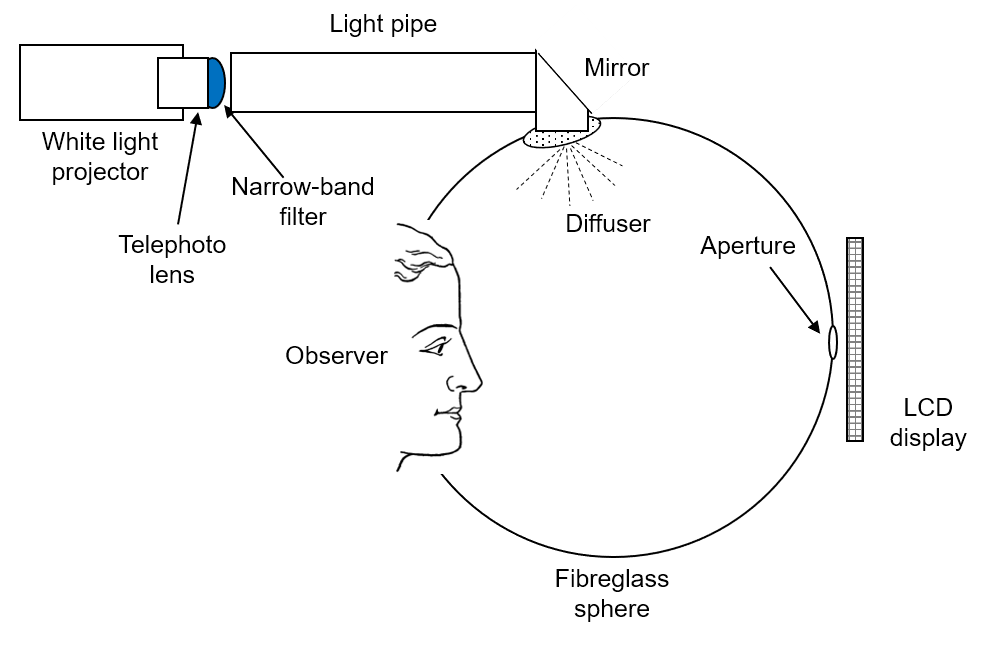
\includegraphics[max width=\textwidth]{figs/LargeSpere/sketch.png}
\caption{The hardware design.}
\label{fig:sketch}
\end{figure}

\begin{figure}[htbp]
%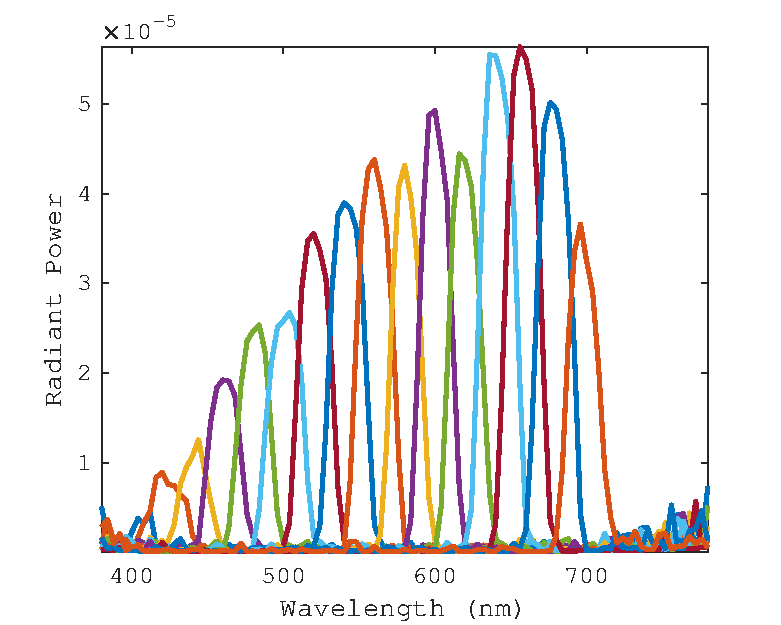
\includegraphics[max width=\textwidth]{figs/LargeSpere/LSillum.pdf}
\caption{The illuminants within the sphere (created by filtering light from a slide projector).}
\label{fig:illum}
\end{figure}

\subsection{Observer task}

The observer sat on one side of the sphere with their face inside the sphere, such that nothing outside of the sphere was visible. On view on the opposite side of the sphere was a circular 4$^{\circ}$ aperture onto an LCD screen, upon which a random colour drawn from ??????%
was visible. It was the observer's task to use two handheld sliders, which controlled the chromaticity of the screen, to make the appearance of the screen achromatic. Once they were happy with the achromacy of the patch, they were to hit a button at which a new random colour would be presented. The first displayed colour was displayed at L* of 85, with subsequent colours descending by 5 L* until 15 L*. This scale was repeated 10 times per session. Per session observers made 10 selections at 16 lightness levels (160 total). Observers performed 16 sessions (2560 selections total). See Figure \ref{fig:ExperimentalPro}.

\begin{figure}[htbp]
%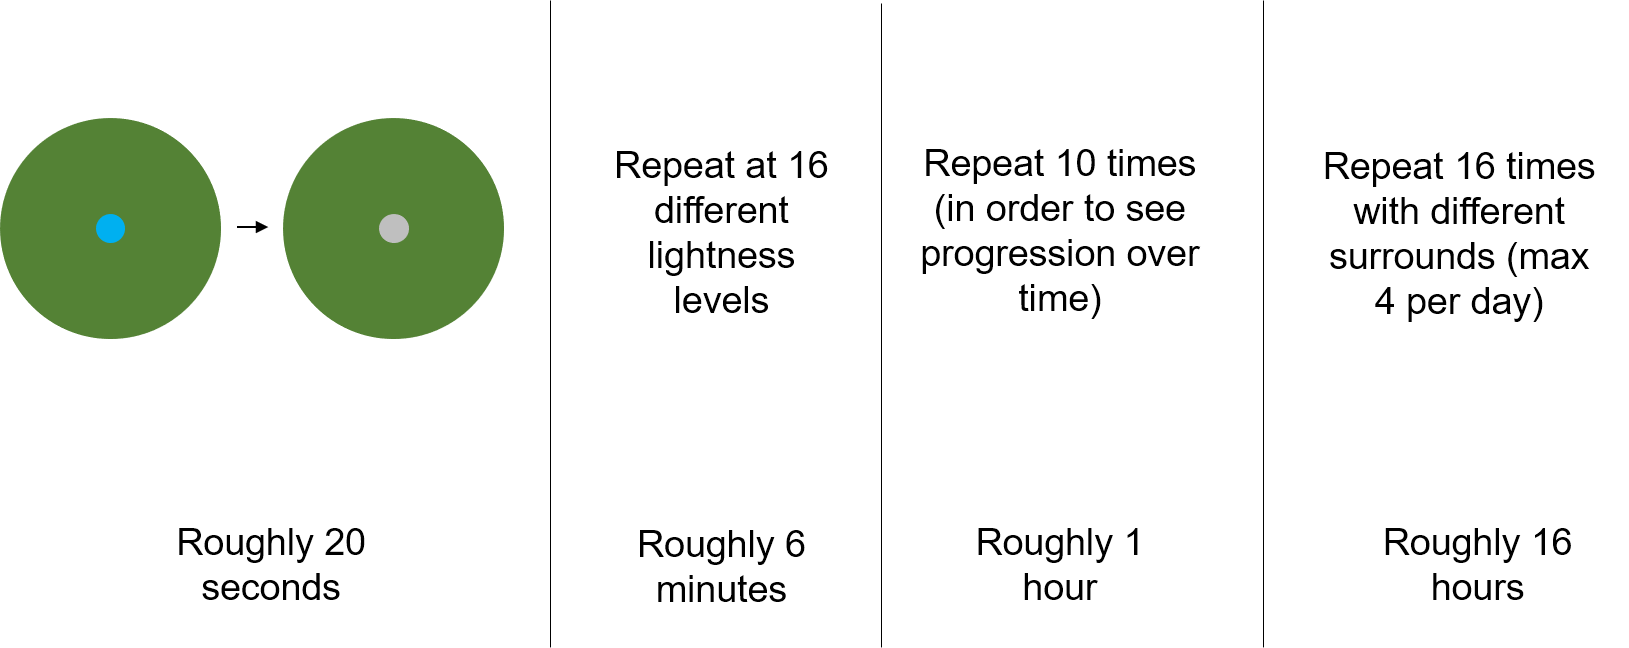
\includegraphics[max width=\textwidth]{figs/LargeSpere/ExperimentalPro.png}
\caption{The experimental protocol.}
\label{fig:ExperimentalPro}
\end{figure}

\subsection{Data Processing}

Two distinct approaches were taken to data processing

\section{Results}
\section{Discussion}
\section{Conclusion}